\documentclass[12pt, a4paper]{article}


% A pretty common set of packages
\usepackage[margin=2.5cm]{geometry}
\usepackage[T1]{fontenc}
\usepackage{graphicx}
\usepackage{amssymb}
\usepackage{amsmath}
\usepackage{color}
\usepackage{booktabs}
\usepackage{multirow}
\documentclass{memoir}
\usepackage{engord}
\usepackage{enumitem}
\usepackage{soul}
\usepackage{multicol}
\usepackage{textcomp}
\usepackage{parskip}
\usepackage{setspace}
\usepackage{titlesec}
\usepackage{subfig}
\usepackage{float}
\usepackage{adjustbox}
\usepackage[demo]{graphicx}
\usepackage{caption}
\usepackage{longtable}
\usepackage{subcaption}
\usepackage{siunitx,booktabs,caption}
\usepackage{listings}
\usepackage[spanish]{babel}
\usepackage[skip=2pt,font=footnotesize,justification=centering]{caption}
\usepackage{natbib}
\usepackage[skip=10pt plus1pt, indent=40pt]{parskip}
\usepackage{parskip}
\usepackage[colorlinks=true, 
    linkcolor=blue,          % color of internal links
    citecolor=blue,        % color of links to bibliography
    filecolor=blue,      % color of file links
    urlcolor=blue]{hyperref}



% Do you prefer Sans Serif fonts?
%\usepackage{sfmath}
%\renewcommand{\familydefault}{\sfdefault} 




% Make some additional useful commands
\newcommand{\ie}{\emph{i.e.}\ }
\newcommand{\eg}{\emph{e.g.}\ }
\newcommand{\etal}{\emph{et al}}
\newcommand{\sub}[1]{$_{\textrm{#1}}$}
\newcommand{\super}[1]{$^{\textrm{#1}}$}
\newcommand{\degC}{$^{\circ}$C}
\newcommand{\wig}{$\sim$}
\newcommand{\ord}[1]{\engordnumber{#1}}
\newcommand{\num}[2]{$#1\,$#2}
\newcommand{\range}[3]{$#1$-$#2\,$#3}
\newcommand{\roughly}[2]{$\sim\!#1\,$#2}
\newcommand{\area}[3]{$#1 \! \times \! #2\,$#3}
\newcommand{\vol}[4]{$#1 \! \times \! #2 \! \times \! #3\,$#4}
\newcommand{\cube}[1]{$#1 \! \times \! #1 \! \times \! #1$}
\newcommand{\figref}[1]{Figure~\ref{#1}}
\newcommand{\eqnref}[1]{Equation~\ref{#1}}
\newcommand{\tableref}[1]{Table~\ref{#1}}
\newcommand{\secref}[1]{Section \ref{#1}}
\newcommand{\XC}{\emph{exchange-correlation}}
\newcommand{\abinit}{\emph{ab initio}}
\newcommand{\Abinit}{\emph{Ab initio}}
\newcommand{\Lonetwo}{L1$_{2}$}
\newcommand{\Dznt}{D0$_{19}$}
\newcommand{\Dtf}{D8$_{5}$}
\newcommand{\Btwo}{B$_{2}$}
\newcommand{\fcc}{\emph{fcc}}
\newcommand{\hcp}{\emph{hcp}}
\newcommand{\bcc}{\emph{bcc}}
\newcommand{\Ang}{{\AA}}
\newcommand{\inverseAng}{{\AA}$^{-1}$}
%\newcommand{\comment}[1]{}
\newcommand{\comment}[1]{\textcolor{red}{[COMMENT: #1]}}
\newcommand{\more}{\textcolor{red}{[MORE]}}
\newcommand{\red}[1]{\textcolor{red}{#1}}

\usepackage{capt-of,graphicx}
\newcounter{pics}

\newcommand\z[2][]{%
  \ifnum\value{pics}=4\par\setcounter{pics}{1}\else\stepcounter{pics}\fi
  \ifhmode\unskip\hfill\fi
  \parbox[t]{.50\textwidth}{%
   \centering\includegraphics[width=\linewidth]{#2}\par
   \ifx\relax#1\relax\else\captionof{figure}{#1}\fi}}

\newcommand{\splitcell}[1]{%
  \begin{tabular}{@{}c@{}}\strut#1\strut\end{tabular}%
}

\begin{document}
\thispagestyle{empty}
	
\begin{figure}[ht]
   \minipage{0.76\textwidth}
		
\includegraphics[width=4cm]{fi.png}
		\label{EscudoUABC}
   \endminipage
   \minipage{0.32\textwidth}
		
\includegraphics[height = 4.5 cm ,width=4.5cm]{unam.png}
		\label{EscudoFC}
	\endminipage
\end{figure}
	
\begin{center}
\vspace{0.8cm}
\LARGE
UNIVERSIDAD NACIONAL AUTÓNOMA DE MÉXICO

\vspace{0.8cm}
\LARGE
FACULTAD DE INGENIERÍA

\vspace{1.7cm}	
\Large
\textbf{Proyecto 2}

\vspace{0.2cm}
\LARGE
Analizador Síntactico

\vspace{1.3cm}
\normalsize	
PRESENTA \\
\vspace{.3cm}
\large
\textbf{Navarrete Zamora Aldo Yael}

\vspace{1.3cm}
\normalsize	
PROFESORA \\
\vspace{.3cm}
\large
\textbf{Laura Sandoval Montaño}

\vspace{1.3cm}
\normalsize	
ASIGNATURA \\
\vspace{.3cm}
\large
\textbf{Compiladores}
\end{center}

\newpage

% --- Objetivos
\section{Objetivos}
Construir, en un mismo programa, los analizadores Léxico y Sintáctico Descendente Recursivo que revisen programas escritos en el lenguaje definido por la gramática definida en la clase.

% --- Descripción
\section{Descripción del problema}

Un compilador se compone de tres analizadores principalmente: 

\begin{enumerate}
  \item \textbf{El analizador léxico}, que se encarga de reconocer cada caracter a la entrada, generar las tablas de símbolos, además de la tabla de cadenas, entre otros. Finalmente, manda esta información en forma de tokens y cadena de átomos al analizador sintáctico.
  \item \textbf{El analizador sintáctico}, el cual se encarga de reconocer la cadena de átomos generada por el analizador léxico y detectar errores de sintaxis dentro de nuestro programa.
  \item \textbf{El analizador semántico}, que utiliza la información en la tabla de símbolos para comprobar la consistencia semántica del programa fuente con la definición del lenguaje. También recopila información sobre el tipo y la guarda en la tabla de símbolos, para usarla más tarde durante la generación de código intermedio.
\end{enumerate}

\textbf{El analizador sintáctico} será el discutido y documentado en este archivo y realizado en este segundo proyecto de la materia de compiladores. Este analizador sintáctico se desarrollará en un archivo distinto al del analizador léxico.

\subsection{Modificaciones al analizador léxico}
Para este proyecto, partimos de la salida que nos generará el analizador léxico una vez procesada la información del archivo de entrada.

Dicho analizador léxico generará las tablas de símbolos y literales, así como los tokens que se transferirán al analizador sintáctico. Este analizador léxico será realizado en lex, LEX es un generador de programas diseñado para procesamiento léxico de flujo de entrada y salida de caracteres. Pero, este analizador tiene algunas restricciones, como por ejemplo:\par
En este documento se describe el problema para afrontar dentro del desarrollo del software que corresponde al analizador sintáctico.

El número de clase es \textbf{inamovible}. 

Además, el analizador léxico tendrá como entrada un archivo con el programa fuente, el cual se indicará desde la línea de comandos al momento de mandar a ejecutar el analizador léxico.

Como delimitador de un componente léxico será uno o vario


\begin{figure}[htpb!]
\centering
  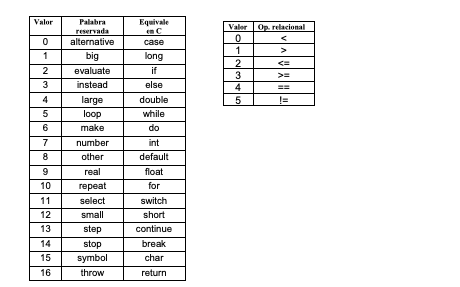
\includegraphics[width=\textwidth]{catalogos.png}
\caption{Catálogos para las palabras reservadas y los operadores relacionales.}
\end{figure}\par


%---- Propuesta de solución
\section{Conjuntos de selección para cada producción}
\begin{center}
  \begin{longtable}{| c | c | }
    \hline
  \multicolumn{2}{|c|}{\textbf{Conjuntos de selección para cada producción}} \\ \hline 
  c.s(1) = \(\{b g # y x\}\)  & c.s(51) = \(\{<\}\) \\   \hline
  c.s(2) = \(\{b g # y x\}\)  & c.s(52) = \(\{l\}\) \\    \hline
  c.s(3) = \(\{ -|\}\)        & c.s(53) = \(\{e\}\) \\    \hline
  c.s(4) = \(\{b g # y x\}\)  & c.s(54) = \(\{d\}\) \\    \hline
  c.s(5) = \(\{b g # y x\}\)  & c.s(55) = \(\{u\}\) \\    \hline
  c.s(6) = \(\{)\}\)  & c.s(56) = \(\{i\}\)\\    \hline
  c.s(7) = \(\{,\}\)  & c.s(57) = \(\{n\}\) \\   \hline
  c.s(8) = \(\{)\}\)  & c.s(58) = \(\{r\}\) \\   \hline
  c.s(9) = \(\{b g # y x i f h w j [ z } c \}\)  & c.s(59) = \(\{s\}\) \\   \hline
  c.s(10) = \(\{i f h w j [ z } c\}\)  & c.s(60) = \(\{n\}\) \\ \hline
  c.s(11) = \(\{b g # y x\}\) & c.s(61) = \(\{i\}\) \\ \hline
  c.s(12) = \(\{b g # y x\}\) & c.s(62) = \(\{r\}\) \\ \hline
  c.s(13) = \(\{b\}\) & c.s(63) = \(\{i\}\) \\ \hline
  c.s(14) = \(\{g\}\) & c.s(64) = \(\{s\}\) \\ \hline
  c.s(15) = \(\{#\}\) & c.s(65) = \(\{i\}\) \\ \hline
  c.s(16) = \(\{y\}\) & c.s(66) = \(\{i\}\) \\ \hline
  c.s(17) = \(\{x\}\) & c.s(67) = \(\{f\}\) \\ \hline
  c.s(18) = \(\{i\}\) & c.s(68) = \(\{h\}\) \\ \hline
  c.s(19) = \(\{;\}\) & c.s(69) = \(\{w\}\) \\ \hline
  c.s(20) = \(\{=\}\) & c.s(70) = \(\{j\}\) \\ \hline
  c.s(21) = \(\{,\}\) & c.s(71) = \(\{[\}\) \\ \hline
  c.s(22) = \(\{n\}\) & c.s(72) = \(\{z\}\) \\ \hline
  c.s(23) = \(\{r\}\) & c.s(73) = \(\{c\}\) \\ \hline
  c.s(24) = \(\{s\}\) & c.s(74) = \(\{ } t : q a o \}\) \\ \hline
  c.s(25) = \(\{;\}\) & c.s(75) = \(\{i f h w j [ z c\}\) \\ \hline
  c.s(26) = \(\{,\}\) & c.s(76) = \(\{w\}\) \\ \hline
  c.s(27) = \(\{i\}\) & c.s(77) = \(\{f\}\) \\ \hline
  c.s(28) = \(\{s\}\) & c.s(78) = \(\{t\}\) \\ \hline
  c.s(29) = \(\{( i n r [\}\) & c.s(79) = \(\{:\}\) \\ \hline
  c.s(30) = \(\{( i n r [\}\) & c.s(80) = \(\{j\}\) \\ \hline
  c.s(31) = \(\{+\}\) & c.s(81) = \(\{i\}\) \\ \hline
  c.s(32) = \(\{-\}\) & c.s(82) = \(\{;\}\) \\ \hline
  c.s(33) = \(\{) ;\}\) & c.s(83) = \(\{i n r s\}\) \\ \hline
  c.s(34) = \(\{( i n r [\}\) & c.s(84) = \(\{;\}\) \\ \hline
  c.s(35) = \(\{*\}\) & c.s(85) = \(\{i\}\) \\ \hline
  c.s(36) = \(\{/\}\) & c.s(86) = \(\{)\}\) \\ \hline
  c.s(37) = \(\{ \ \}\) & c.s(87) = \(\{h\}\) \\ \hline
  c.s(38) = \(\{ \% \}\) & c.s(88) = \(\{a\}\) \\ \hline
  c.s(39) = \(\{^\}\) & c.s(89) = \(\{} o\}\) \\ \hline
  c.s(40) = \(\{+ - ; )\}\) & c.s(90) = \(\{o\}\) \\ \hline
  c.s(41) = \(\{(\}\) & c.s(91) = \(\{}\}\) \\ \hline
  c.s(42) = \(\{i\}\) & c.s(92) = \(\{q\}\) \\ \hline
  c.s(43) = \(\{n\}\) & c.s(93) = \(\{a } o\}\) \\ \hline
  c.s(44) = \(\{r\}\) & c.s(94) = \(\{z\}\) \\ \hline
  c.s(45) = \(\{[\}\) & c.s(95) = \(\{i n r s\}\) \\ \hline
  c.s(46) = \(\{i\}\) & c.s(96) = \(\{)\}\) \\ \hline
  c.s(47) = \(\{n\}\) & c.s(97) = \(\{[\}\) \\ \hline
  c.s(48) = \(\{r\}\) & c.s(98) = \(\{)\}\) \\ \hline
  c.s(49) = \(\{s\}\) & c.s(99) = \(\{ i n r s \}\) \\ \hline
  c.s(50) = \(\{>\}\)   & c.s(100) =\(\{,\}\) \\ \hline
                        & c.s(101) =\(\{)\}\) \\
  \hline
  \end{longtable}
  \end{center}

%----- Ejecución del programa
\section{Ejecución del programa}
El programa se encuentra comentado, con una descripción breve de lo que hace cada una de las funciones. La sangría está muy cuidada y se ve bastante presentable y legible el código.
Para correr el programa, debemos tener instalado flex en nuestro equipo y seguir los siguientes pasos una vez que lo tengamos instalado.

\begin{enumerate}
    \item Abrir en una ventana de terminal la carpeta donde se encuentran todos los archivos.
    \item Una vez dentro de la carpeta correremos el comando \texttt{flex lexical-analyzer.l}
    \item \texttt{gcc lex.yy.c -ly -ll -o lexical-analyzer.out} para compilarlo mediante gcc y tener un archivo de salida ejecutable para un entorno LINUX.
    \item Finalmente, \texttt{./lexical-analyzer.out inputFile.txt} es importante destacar que, el archivo \textit{inputFile.txt} es el archivo de entrada, \textbf{en caso de no teclear ningún archivo de entrada el programa puede manejar este tipo de problema mandando un mensaje de que es necesaria esa entrada por consola.}
\end{enumerate}

Una vez ejecutados los pasos anteriores, podrémos observar \textbf{dos archivos de texto para la salida:}
\begin{enumerate}
    \item El archivo de texto para la generación de los tokens.
    \item El archivo de texto para la la impresión de errores léxicos.
\end{enumerate}

Este último archivo reportará qué expresiones regulares no están definidas por el lenguaje desarrollado.

\section{Conclusiones}
\chapterprecishere{"Hola"}
"\par\raggedleft--- \textup{\textbf{Navarrete Zamora Aldo Yael}}, Estudiante de Ingeniería en Computación}
\end{document}
